%==============================================================================
\chapter{Metodologia}\label{desenvolvimento}
%==============================================================================

Neste capítulo será explicado o método proposto para resolver o problema de \ac{pos} Tagging, juntamente com todas as técnicas utilizadas para seu funcionamento.

\section{Representação das palavras}

Seguimos a ideia explorada em massa pela literatura de representar as palavras através de vetores reais com uma dimensão fixa $d$ definida pelo usuário. Isso será feito utilizando três estratégias já mencionadas: \ac{nlm}, \ac{sg} e \ac{glove}.

Além das \textit{word embeggins}, utilizaremos outras duas \textit{features} importantes no contexto de \ac{pos} Tagging, como capitalização que consegue, na maioria das vezes, distinguir nomeações, e também prefixos, que podem ser usadas para distinguir medidas de tempo, velocidade, etc. 

Em ordem de manter a rede neural homogênea, também iremos transformar cada classe gramatical em um vetor. Com isso poderemos aplicar funções que combinam características do vetor de uma palavra com o vetor de uma classe gramátical.


\section{Pontuações para estrutura gramatical}

Em ordem de classificar palavras em uma sentença, o etiquetador obtém uma janela de palavras de tamanho fixo a cada momento, e transforma as palavras em vetores de \textit{features}, que são então passadas para uma rede neural descrita em \cite{collobert2008unified}. A rede atribui para cada classe gramatical $c \in \gamma$ uma pontuação. A etapa de gerar pontuações para a palavra ocorre no mesmo momento que o treinamento do modelo. A saída para toda a sentença é então passada para o algoritmo de Viterbi \cite{viterbi1967error}, que realiza uma predição estruturada em um tempo polinomial.

Seguimos a estratégia apresentada em \cite{dos2014training} para realizar as pontuações. Nela, a ideia é de que a classe gramatical de uma palavra depende fortemente das palavras vizinhas, o que é verdade para várias aplicações de \ac{pln}, incluindo \ac{pos} Tagging.

Dada uma janela com $t$ palavras $\{w_1, w_2, ..., w_t\}$, que foram transformadas para sua representação vetorial $\{v_1, v_2, ..., v_t\}$, para computar a n-ésima palavra, é centralizada a janela em $n$ e concatena-se todas as palavras da metade à esquerda e da metade à direita em um novo vetor $V_n$ de dimensão $t * d$. Para palavras no começo ou no fim da sentença, é usado vetores com valores fixos para preencher o espaço vazio na janela de palavras. A \autoref{eq:janeladevets} demonstra isso.

\begin{equation} \label{eq:janeladevets}
V_n = \big\{ v_{n - (t-1)/2}, ..., v_n, ..., v_{{n + (t-1)/2}} \big\}
\end{equation}

O novo vetor $V_n$ é então passado para uma rede neural com múltiplas camadas, que computa o resultado $s_c(V_n)$ para cada classe gramatical $c$ da palavra no meio da janela. 

Seguimos a ideia apresentada em \cite{collobert2011natural}, onde é feito um esquema de predição que leva em consideração a estrutura gramatical. O método usa uma pontuação de transição $A_{c,d}$, inicializada com 0, para ir de uma classe $c \in \gamma$ para uma classe $d \in \gamma$ conforme a sequência das palavras. Porém extendemos a notação para funcionar com trigramas: $A_{c,d,e}$. A estrutura $A$ consegue armazenar informações importantes como ``após um pronome é bastante provável que há um verbo''. Depois que a rede produz a pontuação para todas as palavras, a pontuação final de uma sequência de classes gramaticais $c_1^t$ para uma sequência de palavras $w_1^t$, é dada pela \autoref{eq:pontuacaofinal}. $Q$ representa um conjunto com os vetores de palavras que já foram classificados.

\begin{equation} \label{eq:pontuacaofinal}
S(w_1^t, c_1^t) = \sum\limits_{k=1}^{t} \Big( \max_{1 \leq i \leq t, v_i \notin Q} (s_{c_i}(V_i) + A_{c_{i-1}, c_{i}, c_{i+1}}) \Big)
\end{equation}

Após computar isso para cada palavra na sentença, a classe gramatical final é prevista através do algoritmo de Viterbi.


\section{Treinamento}

Para treinar a rede neural, será seguido uma estratégia de aprendizagem guiada por palavras mais fáceis \cite{shen2007guided}. A \autoref{fig:guidedlearning} exemplifica transições mais fáceis em uma frase, onde o peso mais baixo na aresta representa a ordem de execução. Na verdade, cada transição de um nodo para outro conta como uma nova etapa de treinamento. A \autoref{eq:pontuacaofinal} faz esse aprendizado guiado ao realizar a escolha da palavra mais fácil através da maximização das possibilidades que ainda não foram testadas dentro da janela de palavras.

\begin{figure}[htb]
	  \caption{Grafo de transições de palavras mais fáceis}\label{fig:guidedlearning}
	  \begin{center}
	      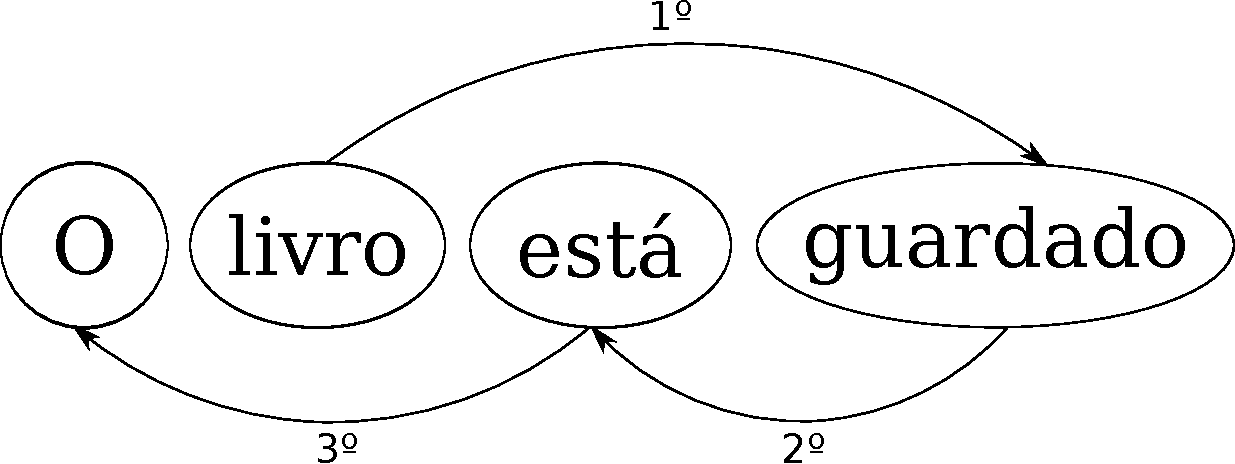
\includegraphics[scale=0.5]{img/guidedlearning.pdf}
	  \end{center}
\end{figure}

Treinar o modelo consiste em ajustar os pesos da rede neural, os valores das \textit{word embeddings} e as pontuações de transição. Após descobrir qual a classe gramatical mais provável para uma palavra $w_n$, o vetor da classe gramatical $z_c$ é composto com o vetor da própria palavra $v_n$ através de uma operação de soma. Essa composição é então armazenada no vetor da própria palavra:

\begin{equation} \label{eq:composicaovets}
v_n = v_n + z_n
\end{equation}


\begin{figure}[htb]
	  \caption{Modelo da rede neural}\label{fig:neuralnetworkfinal}
	  \begin{center}
	      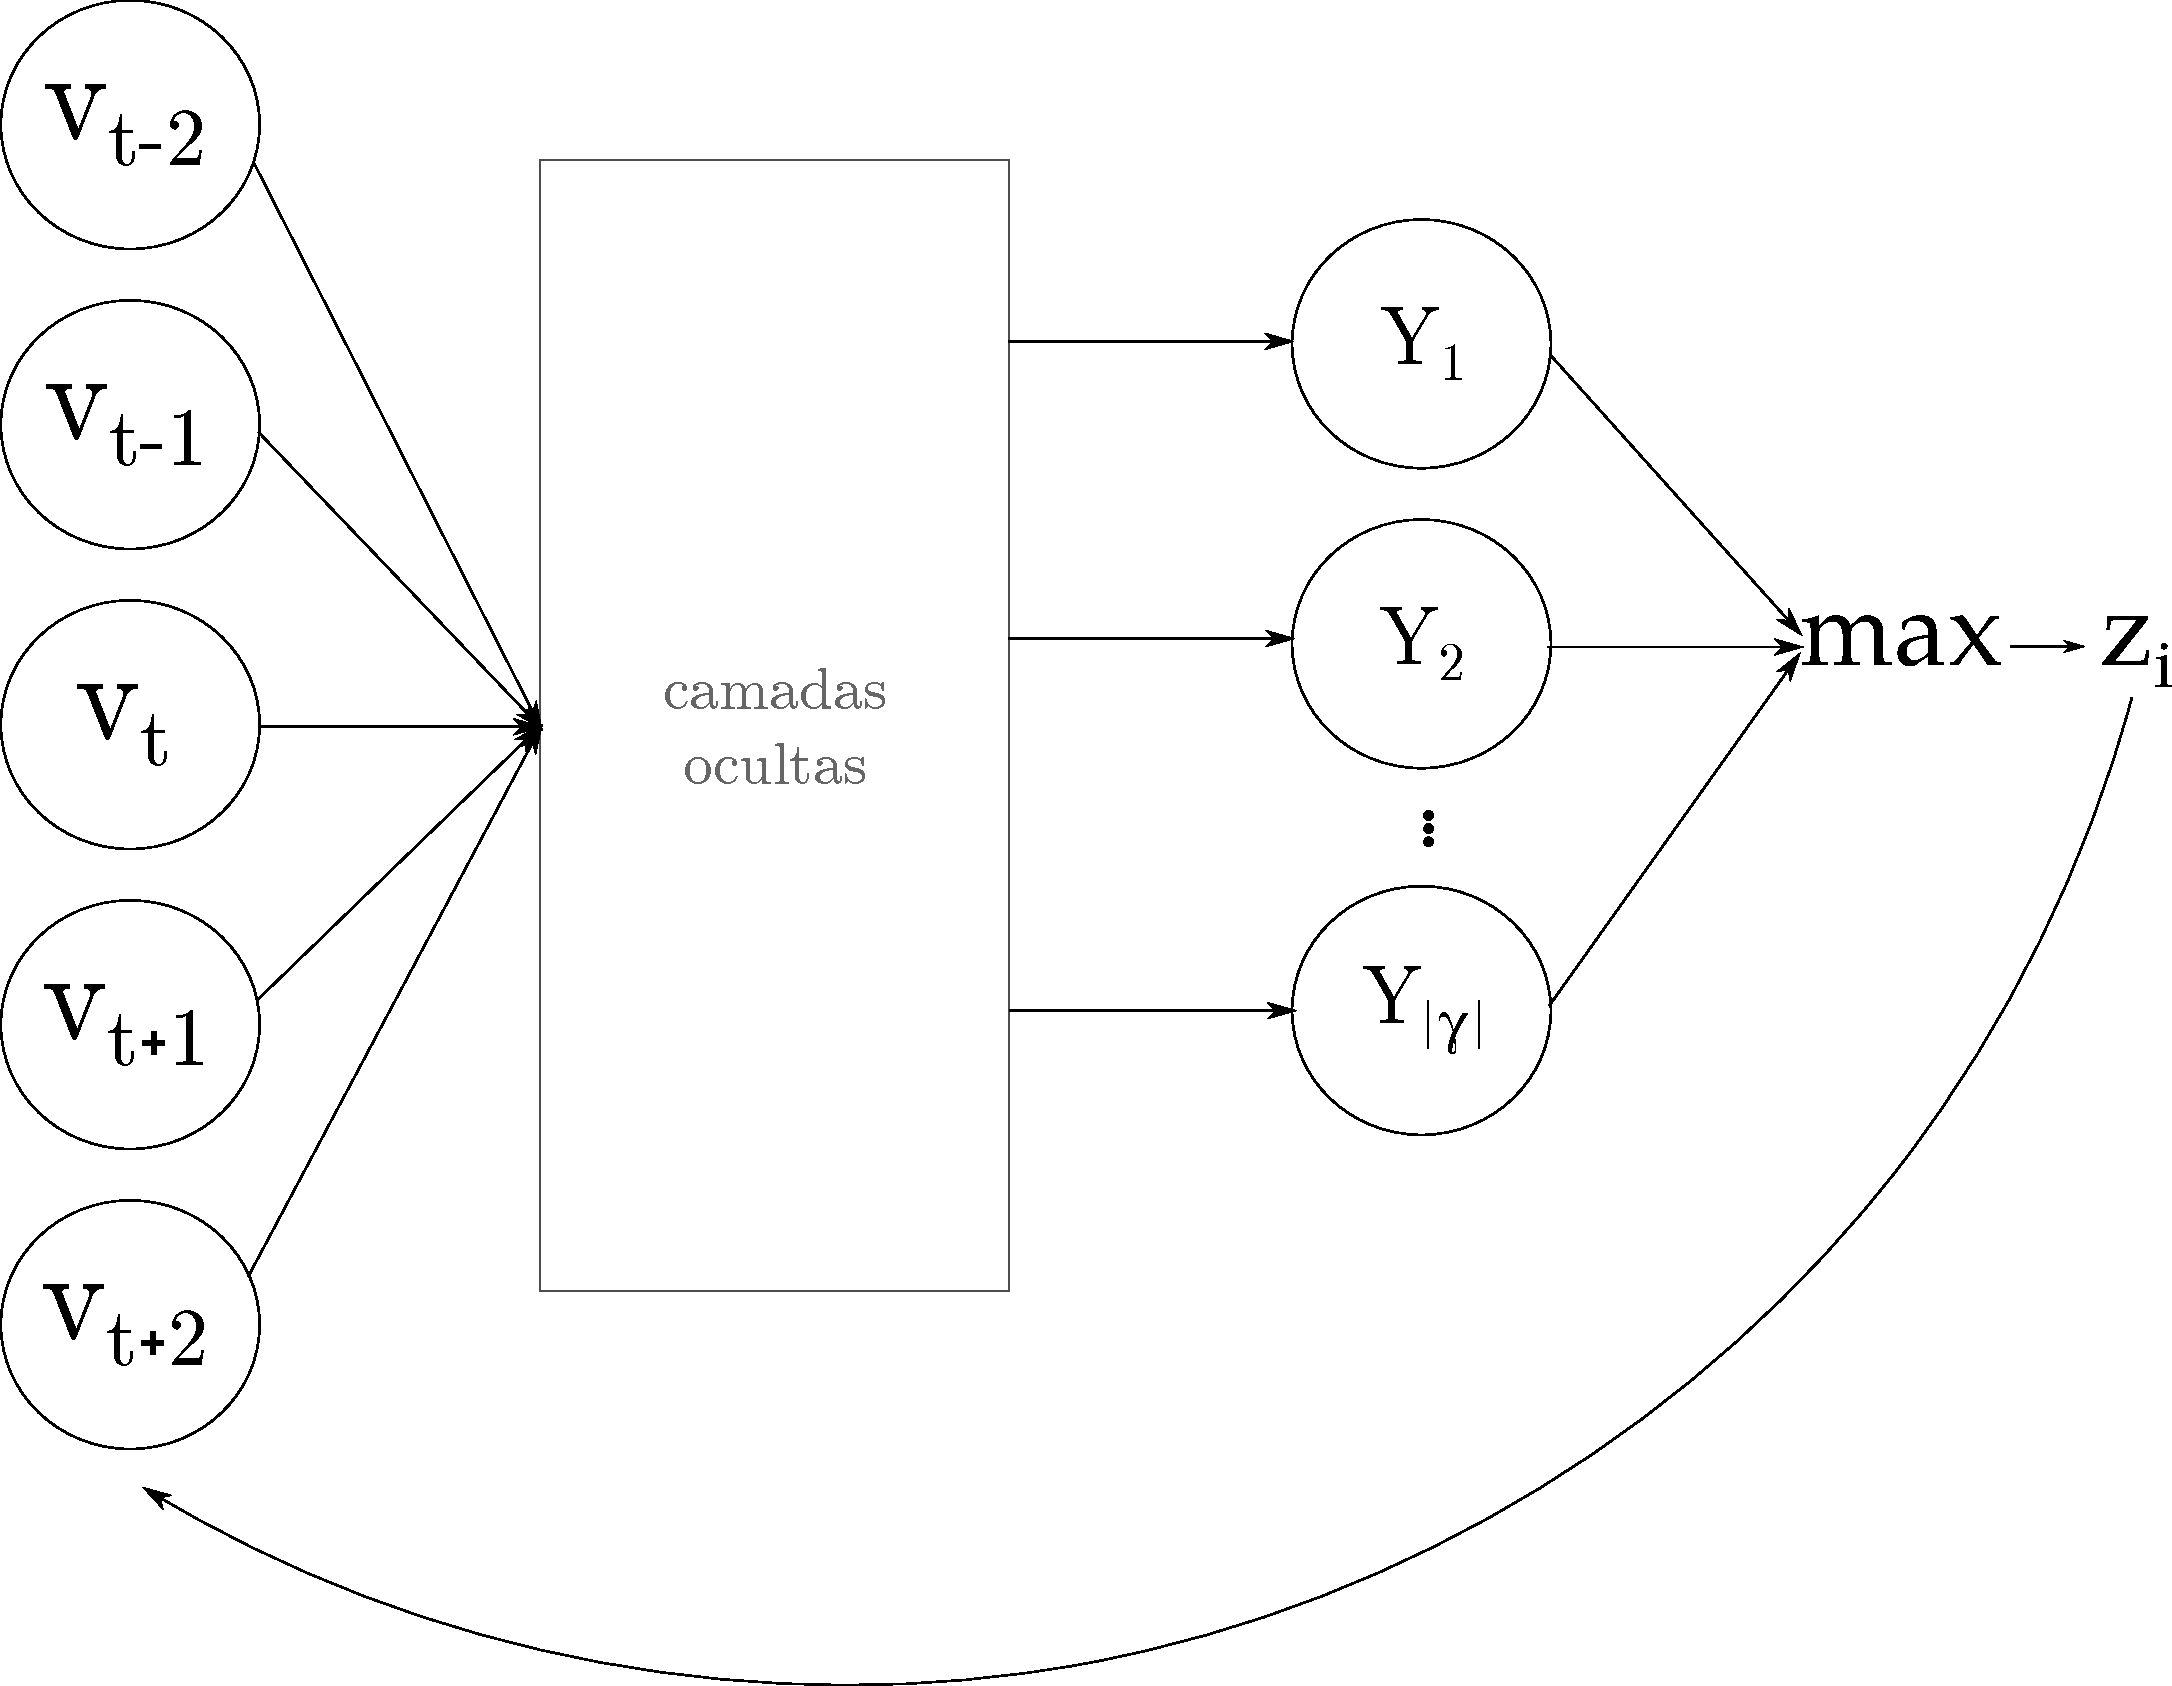
\includegraphics[scale=0.4]{img/neuralnetworkfinal.pdf}
	  \end{center}
\end{figure}

A \autoref{fig:neuralnetworkfinal} ilusta o modelo completo da rede neural. Há um total de 2 camadas ocultas, porém elas foram removidas da imagem por simplificação. A operação \textit{max} no final da rede neural representa a equação \autoref{eq:pontuacaofinal} em conjunto com a predição feita pelo algoritmo de Viterbi. O resultado será o vetor da classe gramatical da palavra mais fácil ainda não analisada $z_i$. Após isso, esse vetor é composto com o vetor da palavra analisada $v_i$ através da \autoref{eq:composicaovets}.

Para treinar a rede neural, todos os ajustamentos são feitos em ordem de maximizar a seguinte equação:

\begin{equation}
\sum\limits_{(w_1^t,c_1^t) \in \Upsilon} P(c_1^t|w_1^t,\theta) \nonumber
\end{equation}

Onde $\Upsilon$ denota o conjuntes dos pares de palavras e classes gramaticais. Seguimos a ideia utilizada por \citeonline{fonseca2015evaluating} e computamos a equação acima utilizando uma operação \textit{softmax}:

\begin{equation}
log(P(c_1^t|w_1^t,\theta)) = S(w_1^t, c_1^t) - log\Bigg(\sum\limits_{u_1^t \in \gamma^t} e^{S(w_1^t, u_1^t)} \Bigg) \nonumber
\end{equation}

E então podemos escrever a função de custo como:

\begin{equation} \label{eq:costfunctionfinalnn}
J(\theta) = log\Bigg(\sum\limits_{u_1^t \in \gamma^t} e^{S(w_1^t, u_1^t)} \Bigg) - S(w_1^t, c_1^t)
\end{equation}

Onde ajustamos os parâmetros da rede utilizando o Gradiente Descendente sobre o primeiro termo da função de custo.  

Mas também queremos maximizar o segundo termo da \autoref{eq:costfunctionfinalnn}. Para isso realizamos um incremento nas pontuações de transição para cada palavra etiquetada corretamente no gradiente descendente:

\begin{equation}
\frac{\partial J(\theta)}{\partial A_{c_{i-1}, c_{i}, c_{i+1}}} \text{ += } 1 \quad \forall i \nonumber
\end{equation}

No fim, rodamos o algoritmo de \textit{Backpropagation} para ajustar os pesos da rede neural até a camada de entrada. 